\pdfinfoomitdate=1
\pdftrailerid{}
\documentclass[12pt]{article}
\usepackage[letterpaper,left=18mm,right=18mm,top=22mm,bottom=20mm,headheight=15pt]{geometry}
\usepackage{tikz,fancyhdr,amsmath}
\usepackage[T1]{fontenc}
\usepackage{lmodern}
\pagestyle{fancy}\fancyhf{}
\fancyhead[L]{\small Week 88 / Packing and kissing circles / Grades K--5}
\fancyfoot[L]{\small Bellingham Math Circle / Week 88 / W88-shared-v1}
\fancyfoot[R]{\small\thepage}
\renewcommand{\headrulewidth}{0.3pt}\renewcommand{\footrulewidth}{0pt}
\setlength{\parindent}{0pt}\setlength{\parskip}{8pt}
\newcommand{\problem}[2]{\par\textbf{Problem #1:} #2\par}
\newcommand{\tray}[1]{\begin{center}\begin{tikzpicture}[x=1mm,y=1mm]
% Four filled strips, whose ink lies entirely outside the stated interior.
\fill[black!75] (-.35,-.35) rectangle (160.35,0);
\fill[black!75] (-.35,#1) rectangle (160.35,{#1+.35});
\fill[black!75] (-.35,0) rectangle (0,#1);
\fill[black!75] (160,0) rectangle (160.35,#1);
\node[above] at (80,{#1+2}) {160 mm};
\node[rotate=90,above] at (-3,{#1/2}) {#1 mm};
\end{tikzpicture}\end{center}}
\newcommand{\lines}[1]{\foreach \y in {1,...,#1}{\par\vspace{10mm}\hrule height .2pt}}
\begin{document}
Disk sizes measure straight across the center. Keep disks flat. They may touch, but must not overlap. In a ring, every outside disk must touch the middle disk.

\problem{1}{Use the 40 mm disks. How many can touch one middle disk at once? Make the biggest ring you can.}

\begin{center}
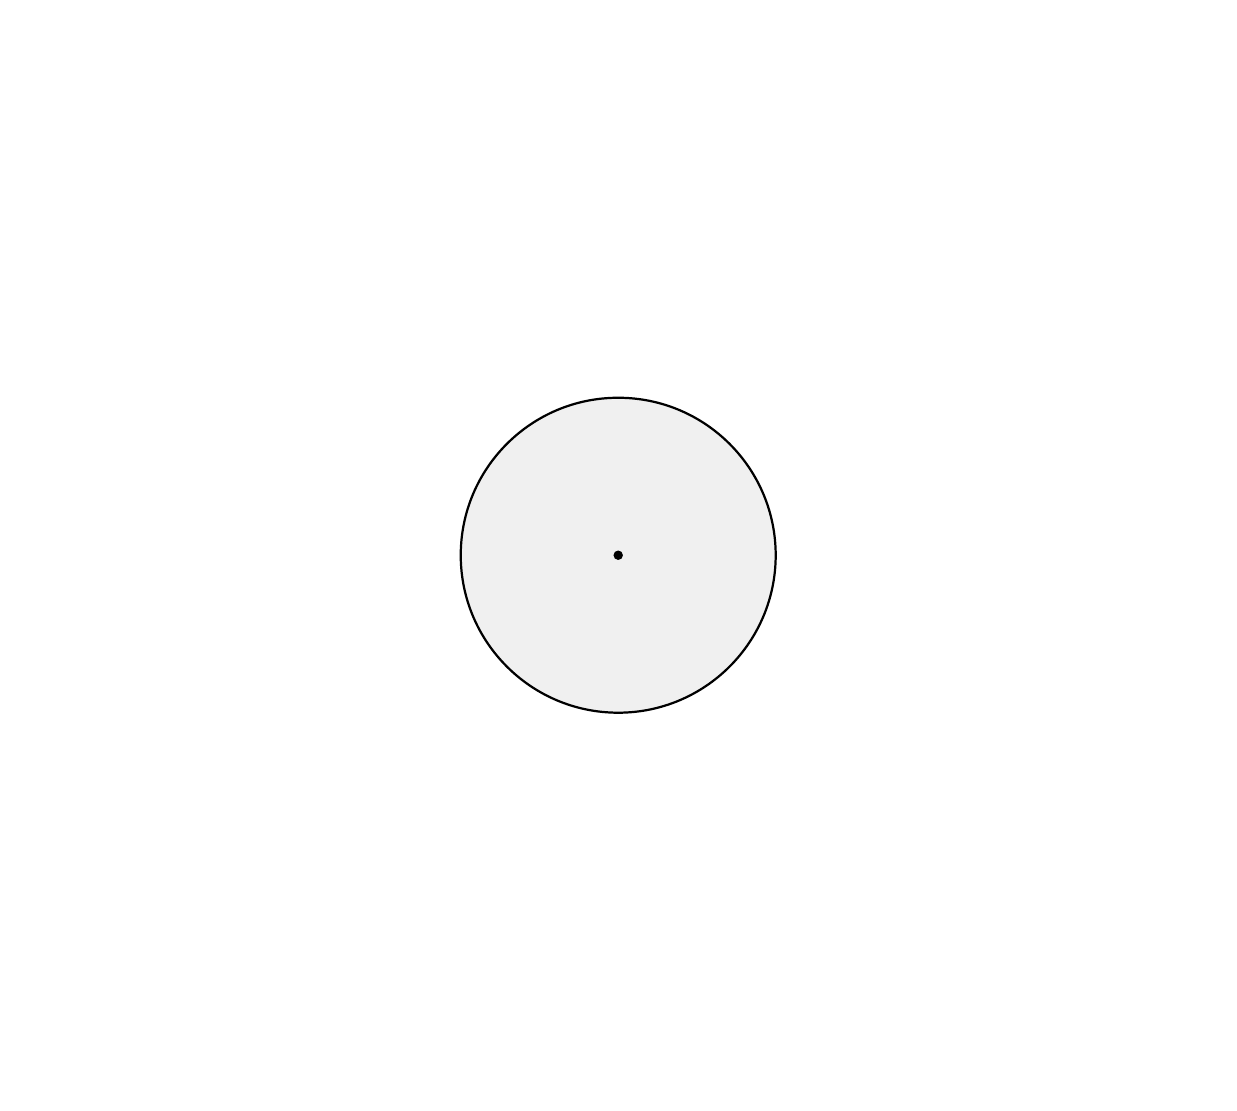
\begin{tikzpicture}[x=1mm,y=1mm]
\path[use as bounding box] (-75,-67) rectangle (75,67);
\draw[thick,fill=black!6] (0,0) circle (20);
\fill (0,0) circle (.6);

\end{tikzpicture}
\end{center}
\vfill
Most outside disks in our ring: \rule{25mm}{.3pt}

\newpage

\problem{2}{How many 40 mm disks can you fit inside this tray? Make a packing that holds as many as you can.}

\vspace{5mm}
\tray{112}
\begin{center}Practical tray: 160 mm $\times$ 112 mm interior\end{center}
\vfill
Our best packing holds \rule{20mm}{.3pt} disks.

\newpage

\problem{3}{Put an 80 mm disk in the middle of your desk mat. Make the biggest ring of 40 mm disks that can touch it.}

\begin{center}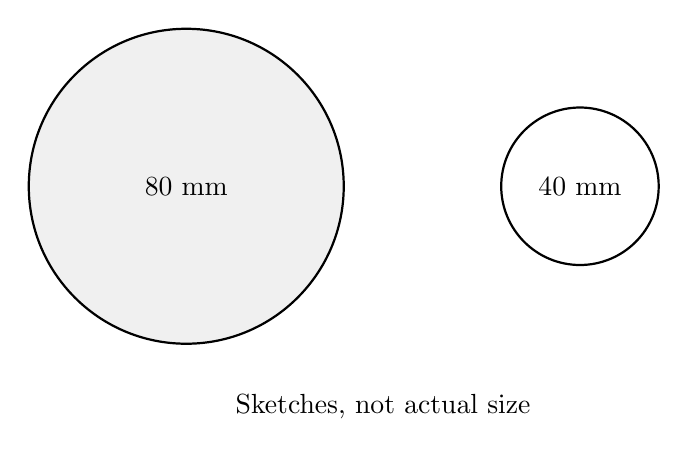
\begin{tikzpicture}[x=1mm,y=1mm]
\draw[thick,fill=black!6] (0,0) circle (20);
\node at (0,0) {80 mm};
\draw[thick] (50,0) circle (10);\node at (50,0) {40 mm};
\node at (25,-28) {Sketches, not actual size};
\end{tikzpicture}\end{center}
Most outside disks: \rule{20mm}{.3pt}
\vspace{10mm}

\problem{4}{Now put a 40 mm disk in the middle. Make the biggest ring of 80 mm disks that can touch it.}

\begin{center}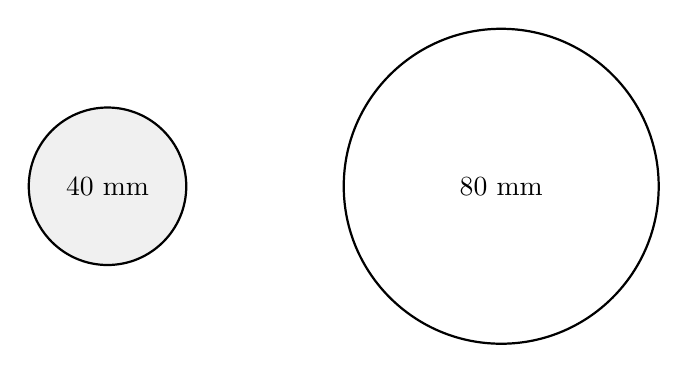
\begin{tikzpicture}[x=1mm,y=1mm]
\draw[thick,fill=black!6] (0,0) circle (10);\node at (0,0) {40 mm};
\draw[thick] (50,0) circle (20);\node at (50,0) {80 mm};
\end{tikzpicture}\end{center}
\vfill
Most outside disks: \rule{20mm}{.3pt}

\newpage

\problem{5}{Make the biggest ring you can using both 40 mm and 80 mm disks on the outside. Try each middle disk below. Every ring must have at least one outside disk of each size.}

\vspace{5mm}
\begin{center}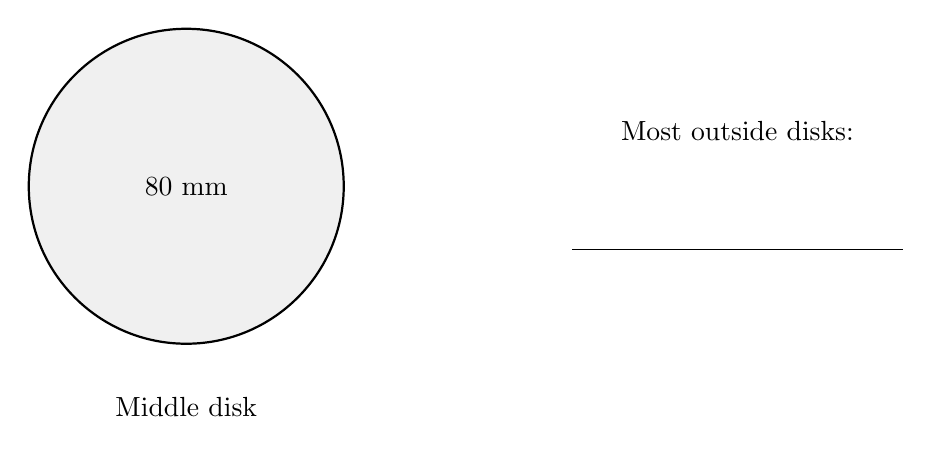
\begin{tikzpicture}[x=1mm,y=1mm]
\draw[thick,fill=black!6] (0,0) circle (20);\node at (0,0) {80 mm};
\node at (70,7) {Most outside disks:};\draw (49,-8)--(91,-8);
\node at (0,-28) {Middle disk};
\end{tikzpicture}\end{center}
\vspace{25mm}
\begin{center}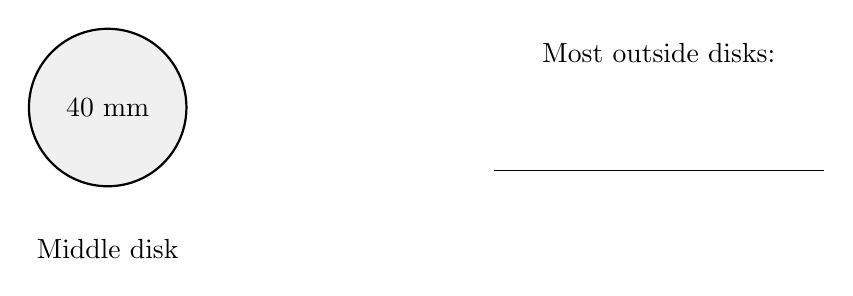
\begin{tikzpicture}[x=1mm,y=1mm]
\draw[thick,fill=black!6] (0,0) circle (10);\node at (0,0) {40 mm};
\node at (70,7) {Most outside disks:};\draw (49,-8)--(91,-8);
\node at (0,-18) {Middle disk};
\end{tikzpicture}\end{center}
\vfill
\begin{center}Sketches, not actual size. Build on your desk mat.\end{center}

\newpage

A radius runs from a circle's center to its edge. For two touching disks, the distance between centers is the sum of their radii.
\begin{center}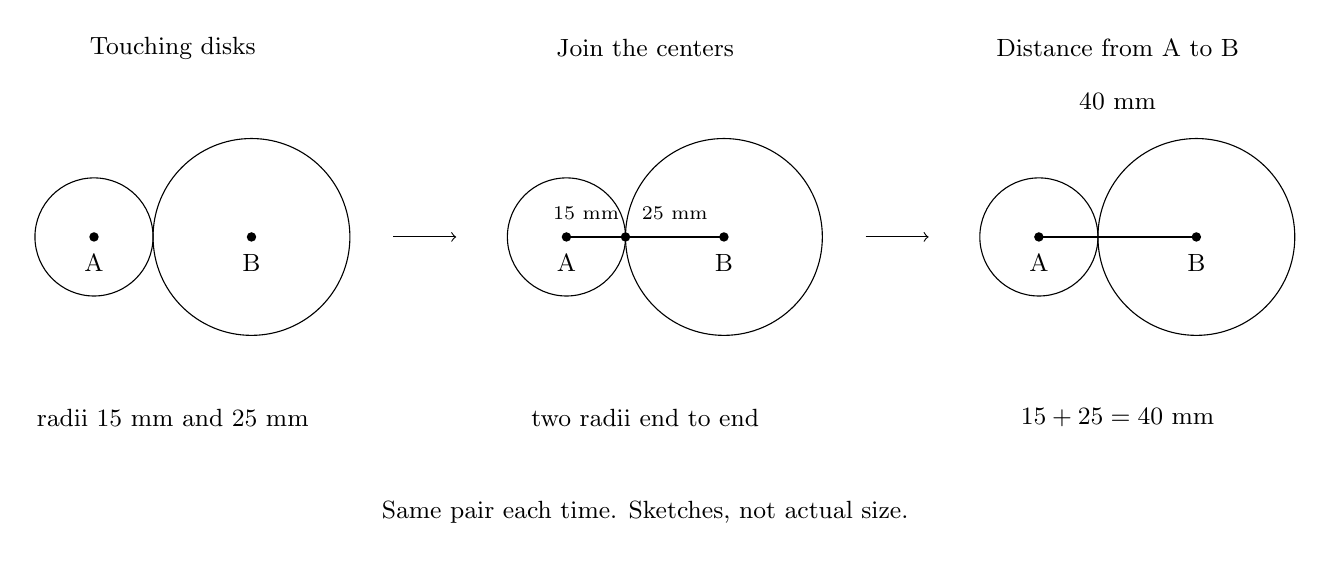
\begin{tikzpicture}[x=1mm,y=1mm,font=\small]
\foreach \x in {0,60,120}{
\draw (\x,0) circle (7.5);\draw ({\x+20},0) circle (12.5);
\fill (\x,0) circle (.6);\fill ({\x+20},0) circle (.6);
\node[below] at (\x,-1) {A};\node[below] at ({\x+20},-1) {B};}
\node at (10,24) {Touching disks};
\node at (10,-23) {radii 15 mm and 25 mm};
\node at (70,24) {Join the centers};
\draw[thick] (60,0)--(80,0);\fill (67.5,0) circle (.6);
\node[above,font=\scriptsize] at (62.5,1) {15 mm};\node[above,font=\scriptsize] at (73.75,1) {25 mm};
\node at (70,-23) {two radii end to end};
\node at (130,24) {Distance from A to B};
\draw[thick] (120,0)--(140,0);
\node[above] at (130,15) {40 mm};
\node at (130,-23) {$15+25=40$ mm};
\draw[->] (38,0)--(46,0);\draw[->] (98,0)--(106,0);
\node at (70,-35) {Same pair each time. Sketches, not actual size.};
\end{tikzpicture}\end{center}

\problem{6}{What is the largest possible ring of 40 mm disks around a 40 mm disk? Explain why one more cannot fit. In every largest ring, must neighboring outside disks touch each other?}

\vspace{3mm}
\begin{center}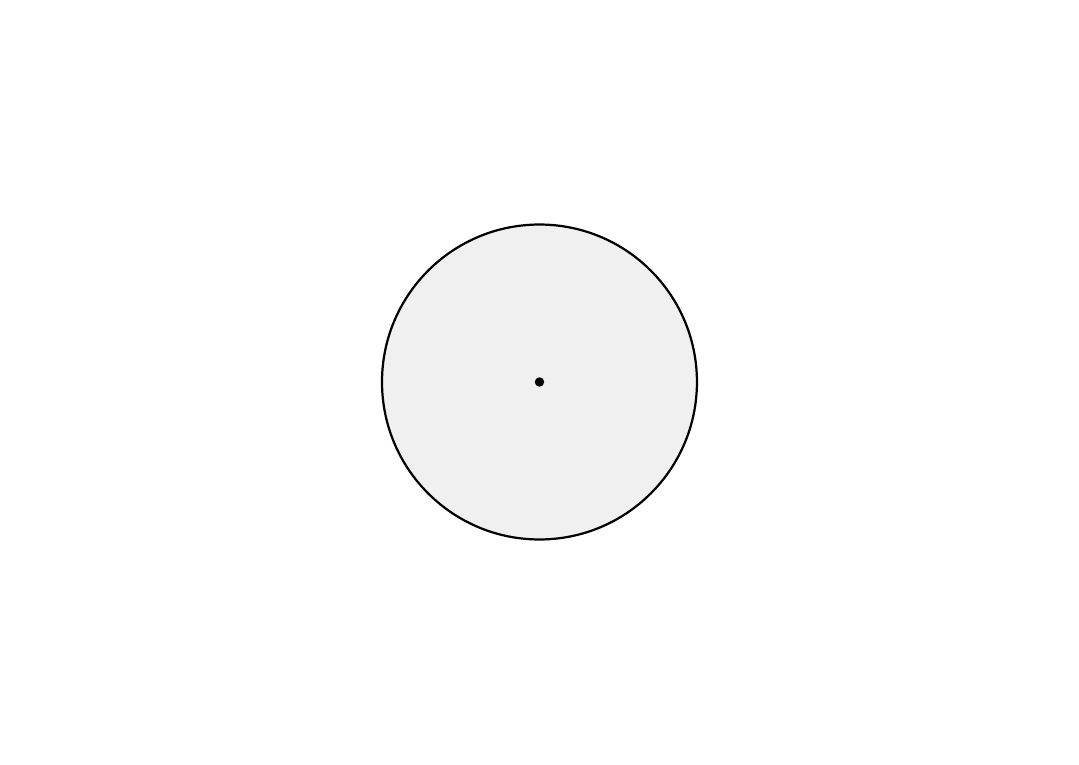
\begin{tikzpicture}[x=1mm,y=1mm]
\path[use as bounding box] (-65,-45) rectangle (65,45);
\draw[thick,fill=black!6] (0,0) circle (20);\fill (0,0) circle (.6);
\end{tikzpicture}\end{center}

\newpage

\problem{7}{Fit eleven 40 mm disks in this exact tray, in three straight horizontal rows: 4, then 3, then 4. Use the center distances to decide whether the disks really fit.}

\vspace{3mm}\tray{110}
\begin{center}Exact tray: 160 mm $\times$ 110 mm interior\end{center}
\vspace{3mm}

\vfill

\newpage

\problem{8}{Can eleven 40 mm disks fit in this tray in three straight horizontal rows: 4, then 3, then 4? Explain your answer for this row arrangement.}

\vspace{3mm}\tray{108}
\begin{center}Exact tray: 160 mm $\times$ 108 mm interior\end{center}
\vspace{3mm}

\problem{9}{Keep the tray 160 mm wide. What is the smallest height that fits those three rows? Give an exact height if you can.}

\vfill

\newpage

\problem{10}{Return to your rings in Problems 3--5. For each one, can you explain why a ring with more outside disks is impossible? Draw the center distances you need.}

\vspace{2mm}
\begin{center}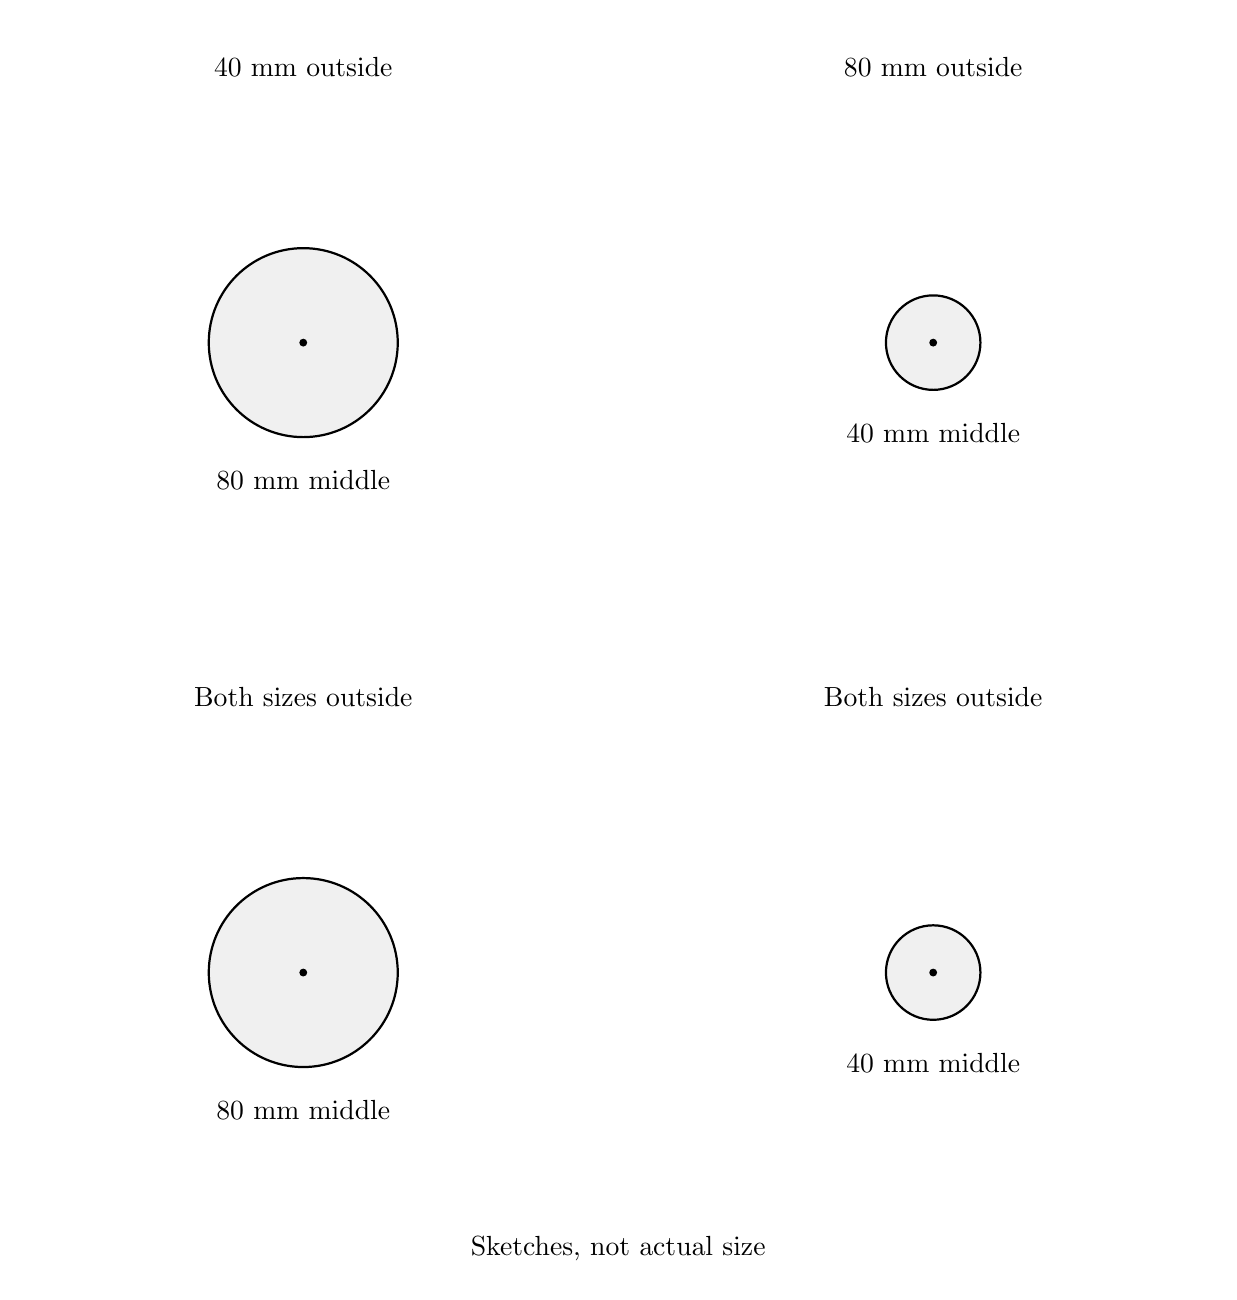
\begin{tikzpicture}[x=1mm,y=1mm]
\foreach \x/\y/\r/\txt in {0/0/12/80,80/0/6/40,0/-80/12/80,80/-80/6/40}{
\draw[thick,fill=black!6] (\x,\y) circle (\r);
\fill (\x,\y) circle (.5);
\node[below] at (\x,{\y-\r-3}) {\txt\ mm middle};}
\node at (0,35) {40 mm outside};
\node at (80,35) {80 mm outside};
\node at (0,-45) {Both sizes outside};
\node at (80,-45) {Both sizes outside};
\node at (40,-115) {Sketches, not actual size};
\path[use as bounding box] (-35,40) rectangle (115,-118);
\end{tikzpicture}\end{center}

\problem{11}{When all the outside disks have the same size, what rule links the two disk sizes to the largest possible ring?}

\vfill
\end{document}
